%Version 3.1 December 2024
% See section 11 of the User Manual for version history
%
%%%%%%%%%%%%%%%%%%%%%%%%%%%%%%%%%%%%%%%%%%%%%%%%%%%%%%%%%%%%%%%%%%%%%%
%%                                                                 %%
%% Please do not use \input{...} to include other tex files.       %%
%% Submit your LaTeX manuscript as one .tex document.              %%
%%                                                                 %%
%% All additional figures and files should be attached             %%
%% separately and not embedded in the \TeX\ document itself.       %%
%%                                                                 %%
%%%%%%%%%%%%%%%%%%%%%%%%%%%%%%%%%%%%%%%%%%%%%%%%%%%%%%%%%%%%%%%%%%%%%

%%\documentclass[referee,sn-basic]{sn-jnl}% referee option is meant for double line spacing

%%=======================================================%%
%% to print line numbers in the margin use lineno option %%
%%=======================================================%%

%%\documentclass[lineno,pdflatex,sn-basic]{sn-jnl}% Basic Springer Nature Reference Style/Chemistry Reference Style

%%=========================================================================================%%
%% the documentclass is set to pdflatex as default. You can delete it if not appropriate.  %%
%%=========================================================================================%%

%%\documentclass[sn-basic]{sn-jnl}% Basic Springer Nature Reference Style/Chemistry Reference Style

%%Note: the following reference styles support Namedate and Numbered referencing. By default the style follows the most common style. To switch between the options you can add or remove “Numbered” in the optional parenthesis. 
%%The option is available for: sn-basic.bst, sn-chicago.bst%  
 
%%\documentclass[pdflatex,sn-nature]{sn-jnl}% Style for submissions to Nature Portfolio journals
%%\documentclass[pdflatex,sn-basic]{sn-jnl}% Basic Springer Nature Reference Style/Chemistry Reference Style
\documentclass[pdflatex,sn-mathphys-num]{sn-jnl}% Math and Physical Sciences Numbered Reference Style
%%\documentclass[pdflatex,sn-mathphys-ay]{sn-jnl}% Math and Physical Sciences Author Year Reference Style
%%\documentclass[pdflatex,sn-aps]{sn-jnl}% American Physical Society (APS) Reference Style
%%\documentclass[pdflatex,sn-vancouver-num]{sn-jnl}% Vancouver Numbered Reference Style
%%\documentclass[pdflatex,sn-vancouver-ay]{sn-jnl}% Vancouver Author Year Reference Style
%%\documentclass[pdflatex,sn-apa]{sn-jnl}% APA Reference Style
%%\documentclass[pdflatex,sn-chicago]{sn-jnl}% Chicago-based Humanities Reference Style

%%%% Standard Packages
%%<additional latex packages if required can be included here>

\usepackage{graphicx}%
\usepackage{multirow}%
\usepackage{amsmath,amssymb,amsfonts,amsthm}%
\usepackage{amsthm}%
\usepackage{mathrsfs}%
\usepackage[title]{appendix}%
\usepackage{xcolor}%
\usepackage{textcomp}%
\usepackage{manyfoot}%
\usepackage{booktabs}%
\usepackage{makecell}%
\usepackage{algorithm}%
\usepackage{algorithmicx}%
\usepackage{algpseudocode}%
\usepackage{listings}%
\usepackage{tikz}
\usetikzlibrary{positioning, calc, arrows.meta}
\usetikzlibrary{arrows.meta, positioning, fit, backgrounds}


\definecolor{slate50}{HTML}{F8FAFC}
\definecolor{slate300}{HTML}{CBD5E1}
\definecolor{slate600}{HTML}{475569}
\definecolor{slate800}{HTML}{0F172A}

\definecolor{amber50}{HTML}{FFFBEB}
\definecolor{amber700}{HTML}{B45309}

\definecolor{emerald50}{HTML}{ECFDF5}
\definecolor{emerald700}{HTML}{047857}

\definecolor{rose50}{HTML}{FEF2F2}
\definecolor{rose700}{HTML}{B91C1C}


\usepackage{bm}
\usepackage{microtype}
\usepackage{enumitem}
 
\newtheorem{proposition}{Proposition}
\newcommand{\YES}{\mathrm{YES}}
\newcommand{\NO}{\mathrm{NO}}
\newcommand{\ind}{\mathbf{1}}
\newcommand{\Prob}{\mathbb{P}}

\usepackage{xr-hyper}    
\usepackage{hyperref}    
\usepackage{zref-base}

\makeatletter
\newcommand*{\addFileDependency}[1]{% 
  \typeout{(#1)}
  \@addtofilelist{#1}
  \IfFileExists{#1}{}{\typeout{No file #1.}}
}
\makeatother

\newcommand*{\myexternaldocument}[1]{% 
  \externaldocument{#1}%
  \addFileDependency{#1.tex}%
  \addFileDependency{#1.aux}%
}

\myexternaldocument{SI}

%%%%%=============================================================================%%%%
%%%%  Remarks: This template is provided to aid authors with the preparation
%%%%  of original research articles intended for submission to journals published 
%%%%  by Springer Nature. The guidance has been prepared in partnership with 
%%%%  production teams to conform to Springer Nature technical requirements. 
%%%%  Editorial and presentation requirements differ among journal portfolios and 
%%%%  research disciplines. You may find sections in this template are irrelevant 
%%%%  to your work and are empowered to omit any such section if allowed by the 
%%%%  journal you intend to submit to. The submission guidelines and policies 
%%%%  of the journal take precedence. A detailed User Manual is available in the 
%%%%  template package for technical guidance.
%%%%%=============================================================================%%%%

%% as per the requirement new theorem styles can be included as shown below
\theoremstyle{thmstyleone}%
\newtheorem{theorem}{Theorem}%  meant for continuous numbers
%%\newtheorem{theorem}{Theorem}[section]% meant for sectionwise numbers
%% optional argument [theorem] produces theorem numbering sequence instead of independent numbers for Proposition
%%\newtheorem{proposition}{Proposition}% to get separate numbers for theorem and proposition etc.

\theoremstyle{thmstyletwo}%
\newtheorem{example}{Example}%
\newtheorem{remark}{Remark}%

\theoremstyle{thmstylethree}%
\newtheorem{definition}{Definition}%

\raggedbottom
%%\unnumbered% uncomment this for unnumbered level heads

\begin{document}

\title[Article Title]{Do We Need the Largest LLMs for Every Clinical Decision?}

\author*[1,2]{\fnm{Ali H.} \sur{Lazem}}\email{lhl23prg@bangor.ac.uk}
\author[1]{\fnm{William} \sur{Teahan}}\email{w.j.teahan@bangor.ac.uk}

\affil*[1]{\orgdiv{School of Computer Science and Engineering},
\orgname{Bangor University}, \orgaddress{\city{Bangor},
\postcode{LL57 2DG}, \state{Gwynedd}, \country{United Kingdom}}}
\affil[2]{\orgname{University of Thi-Qar}, \orgaddress{\city{Nasiriyah},
\postcode{64001}, \country{Iraq}}}

%%==================================%%
%% Sample for unstructured abstract %%
%%==================================%%

\abstract{Large clinical language models often require multi-GPU infrastructure, which limits local
deployment. We introduce CERTA, a decision-level statistical certificate that determines when a
quantized model may substitute for its BF16 reference and escalates uncertifiable
decisions to that reference. Across eleven general and domain-adapted models from three families
(7--72B), evaluated on 2{,}500 clinical-verification decisions constructed from real de-identified
patient contexts (2{,}484 patients) with patient-disjoint calibration and testing, 8-bit quantization
certified at least 99.8\% of decisions for every model. Under a class-conditional guarantee, a 4-bit
scheme reduced the certified footprint to about a quarter of the BF16 size for Qwen2.5-72B and
HuatuoGPT-o1-72B, moving 70--72B models from a measured 142--146\,GB across two 80\,GB GPUs to
41--43\,GB, within the capacity of a single 48\,GB GPU. Independent
disease named-entity benchmarking against human annotations showed the deployed configurations
largely preserved disease named-entity F1. CERTA converts compression from a fixed precision choice into a
risk-controlled deployment policy.
}



\keywords{clinical decision support; large language models; model quantization and compression; conformal risk control; selective prediction (certify-or-escalate); class-conditional (Mondrian) certification; on-premises / single-GPU inference.
}

%%\pacs[JEL Classification]{D8, H51}

%%\pacs[MSC Classification]{35A01, 65L10, 65L12, 65L20, 65L70}

\maketitle

Large language models are increasingly capable on clinical text~\cite{singhal2023clinical,thirunavukarasu2023medicine}, yet the most capable open-weight
models are also among the largest, and running a 70-billion-parameter model in bfloat16
requires accelerator memory that can exceed the capacity available in many healthcare and research settings. A single such
model in its native precision occupies well over one hundred gigabytes and spans two high-end
datacenter GPUs. This puts a practical barrier between the models that perform best on clinical
language and the settings where clinical data is most sensibly kept, at the point of care, inside an
institution's firewall, on a modest local server.
 
Quantization is the usual route to a smaller model. Lowering the numerical precision of the weights
shrinks the memory footprint, sometimes several-fold, and a large literature reports that aggregate
accuracy stays close to the original after quantization~\cite{frantar2023gptq,dettmers2022llmint8,dettmers2023qlora,lin2024awq}. Aggregate accuracy, however, is the wrong
currency for a clinical decision. Two models can match on a benchmark score while disagreeing on
individual cases, and in a verification or triage step it is the individual decision, accept this
finding or reject it, that carries the consequence. A method that preserves an average can still
flip the specific calls that matter, and standard benchmarks offer no per-decision guarantee that
the smaller model may stand in for the larger one.
 
Our question is therefore narrower and more operational than whether the compressed model is still
accurate: for the decision in front of us, can the compressed model be used in place of the
BF16 reference model without changing the decision, and can that substitution be controlled at a
stated error rate? Posed this way, the choice of precision stops being a fixed global setting and
becomes a per-decision, per-model question with a testable answer.
 
We answer it with CERTA, a procedure that certifies or escalates each decision (Fig.~\ref{fig:architecture}). From the compressed
model's own output, CERTA computes a finite-sample statistical certificate~\cite{angelopoulos2021ltt,angelopoulos2023gentle,angelopoulos2024crc} that its decision agrees
with the BF16 reference at a chosen risk level. Decisions that clear the certificate are
served by the compressed model, and the rest are escalated to the reference. Repeating this across
bit-widths and quantizers gives, for each model, the least costly configuration the certificate will
accept at a given risk, which we call its certified compression frontier. Because a clinical
accept/reject decision has two sides with different consequences, the deployable policy controls the
reject decision separately from the accept decision.
 
Across eleven models from three families, spanning 7 to 72 billion parameters and including both
general-purpose and clinically adapted checkpoints, evaluated on 2{,}500 verifier decisions constructed from real de-identified patient contexts
drawn from 2{,}484 patients, eight-bit quantization was certified for every model, and a four-bit
scheme reduced the certified footprint to a quarter of the BF16 size for the strongest
models, moving a 72-billion-parameter model from two large accelerators to one. The question in our
title, whether the largest model is needed for every clinical decision, has a concrete answer: for
most decisions a compressed model suffices and can be certified to do so, and the certificate
identifies the minority that must be referred to the full model.



\section*{Results}
 
We evaluated CERTA on the accept/reject decision of an in-house clinical verifier, using 2{,}500
decisions drawn from 2{,}484 patients and split patient-disjointly into 1{,}250 for calibration and
1{,}250 for held-out test, across eleven models, two quantizers and risk budgets from $1\%$ to
$10\%$.
 
\subsection*{Eight-bit substitution is certified across all evaluated models}
 
At $8$-bit, the certificate accepted the quantized model on essentially every decision (the certify-or-escalate policy is shown in Fig.~\ref{fig:architecture}). Certified
coverage was $99.8\%$ to $100\%$ for all eleven models, with empirical certified-set agreement of
$97.8\%$ to $99.5\%$, at half the weight memory of the bfloat16 reference (Fig.~\ref{fig:landscape}a; per-configuration
certified coverage and agreement for every model are in Supplementary Table~\ref{stab:perconfig}). The result was uniform
across general-purpose and clinically adapted checkpoints, across the Llama, Qwen and Mistral
families, and across the $7$B to $72$B range, and the earlier fragility we had observed on a
smaller synthetic set did not survive the move to real prompts. Across configurations, certified coverage fell well below raw decision preservation, because the certificate rejects low-margin cases (Fig.~\ref{fig:landscape}b). At $6$-bit the certificate remained
strong for nine of the eleven models, each with at least $98\%$ certified coverage (for example
MMed-Llama-3-8B at $98.2\%$); the two exceptions were MMed-Llama-3.1-70B at $93.6\%$ and
BioMistral-7B at $80.3\%$.
 
Round-to-nearest at $4$-bit, by contrast, was strongly model-dependent. Certified coverage ranged
from $0\%$ for MMed-Llama-3-8B to $91$--$94\%$ for HuatuoGPT-o1-72B and Qwen2.5-72B, with the
medical fine-tunes of the shared Llama-3 backbone falling across the whole interval. This split, an
$8$-bit result that holds for every model against a $4$-bit result that holds for only some, is the
problem the rest of the study addresses: a fixed precision is either too conservative for the robust
models or fails the prespecified decision-risk criterion for the fragile ones.
 
\subsection*{The certified compression frontier is model and quantizer specific}
 
A real $4$-bit quantizer changed the picture. NF4 raised raw $4$-bit decision preservation for all
eleven models relative to round-to-nearest, and its certified coverage at $4$-bit ranged from
$82.2\%$ to $100\%$. Qwen2.5-72B and HuatuoGPT-o1-72B certified at $100\%$, and the domain
fine-tunes that round-to-nearest had failed now certified at high coverage under NF4, OpenBioLLM-70B
at $98.1\%$, Med42-70B at $97.5\%$, MMed-Llama-3.1-70B at $96.9\%$ and BioMistral-7B at $95.8\%$ (Fig.~\ref{fig:quantizer}).

Taking the lower envelope over the two quantizers at a $5\%$ risk budget, the certified compression
frontier selected NF4 for ten of the eleven models and settled between $25.0\%$ and $37.5\%$ of the
bfloat16 size. Qwen2.5-72B and HuatuoGPT-o1-72B reached the $4$-bit floor at $25.0\%$, a fourfold
reduction, with no escalation. Only Llama-3.3-70B preferred round-to-nearest at $6$-bit ($37.5\%$)
over its NF4 $4$-bit point, because its NF4 coverage ($82.2\%$) sat just below the break-even
coverage that would justify the more aggressive setting. This break-even structure, in which moving
from $k$ to $k'$ bits reduces amortized size only once certified coverage exceeds
$(16-k)/(16-k')$, accounts for the entire pattern of bit-width selection and for why the frontier
tends to rest at $4$-bit rather than lower. The two quantizers were complementary rather than
redundant, and the certificate, not a prior preference for one scheme, chose between them.
 
\subsection*{A risk budget sets the minimum deployable footprint}
 
Sweeping the risk budget turned the frontier into a per-model risk--resource curve. At a stringent
$1\%$ disagreement budget every one of the eleven models still had a certified operating point,
between $31.2\%$ and $48.2\%$ of bfloat16 size. At $5\%$ the range was $25.0\%$ to $37.5\%$, and at
$10\%$ it tightened to $25.0\%$ to $30.2\%$, with ten of the eleven models at the $4$-bit floor. The
curves were smooth and monotonic, so an operator can read the deployable footprint directly against
whatever disagreement risk a setting permits (Fig.~\ref{fig:risk}a; the frontiers for all eleven
models appear in Supplementary Fig.~\ref{sfig:frontiers}, and are robust to the confidence budget,
calibration size, threshold-grid resolution and the choice of calibration/test split, Supplementary
Figs~\ref{sfig:robust} and~\ref{sfig:gridsplit} and Supplementary Tables~\ref{stab:conf},
\ref{stab:calsize}, \ref{stab:grid} and~\ref{stab:split}).
 
The certificate was well calibrated in aggregate. At each model's deployed operating point the
disagreement observed on the held-out test set stayed at or below the target budget for every model
at $\alpha\le 5\%$ (observed $0.9\%$ to $4.8\%$ at $\alpha=5\%$, and $0.0\%$ to $0.6\%$ at
$\alpha=1\%$); the only exceedance was Med42-70B at $\alpha=10\%$, at $10.5\%$ against a $10\%$
target, within the confidence slack of the procedure (Fig.~\ref{fig:risk}b).
 
\subsection*{Class-conditional certification protects the reject decision}
 
Aggregate calibration, however, does not imply calibration within a decision class, and the
distinction matters clinically because a reject (NO) decision suppresses an unsupported output.
Partitioning by the quantized model's own decision, the marginal certificate violated the per-class
$5\%$ budget for six model-classes at NF4 $4$-bit, four of them on the reject side. Among
predicted-NO decisions the observed disagreement reached $17.4\%$ for OpenBioLLM-70B, $10.0\%$ for
MMed-Llama-3-8B, $6.1\%$ for MMed-Llama-3.1-70B and $6.1\%$ for Mistral-7B; the accept-side violations
were Llama-3-70B-base at $6.9\%$ and Qwen2.5-72B at $5.2\%$. These failures were not specific to NF4:
at round-to-nearest $8$-bit the reject class of MMed-Llama-3.1-70B still exceeded the budget. A high
aggregate coverage concealed these.
 
Class-conditional (Mondrian) certification removed them (Fig.~\ref{fig:risk}c). With a separate threshold per predicted
class, every decision class was brought to at most the target risk or escalated in full:
OpenBioLLM-70B, MMed-Llama-3.1-70B and BioMistral-7B escalated their entire reject class rather than certify it
unsafely, for two distinct reasons: the reject classes of OpenBioLLM-70B and BioMistral-7B are too small
to certify at the target risk, whereas MMed-Llama-3.1-70B has adequate calibration resolution but too
many reject-side disagreements for any threshold to clear the target (Supplementary
Table~\ref{stab:classres} and Supplementary Fig.~\ref{sfig:classres}). The remaining reject classes were certified at reduced coverage under a stricter
per-class threshold (MMed-Llama-3-8B, for instance, at $35.1\%$ reject-class coverage), while the
accept class continued to certify at high coverage (MMed-Llama-3.1-70B at $96.5\%$). Under this
clinically appropriate policy, controlled jointly across both classes at confidence $1-\delta$, the
frontier at $\alpha=5\%$ spanned $25.8\%$ to $40.2\%$ of bfloat16 size (Table~\ref{tab:frontier}). Whereas the
marginal frontier selected NF4 for ten of the eleven models, the stricter class-conditional policy
selected NF4 for all eleven, and at $\alpha=5\%$ the compressed model served most decisions,
escalating only $1.1\%$ (Qwen2.5-72B) to $20.2\%$ (MMed-Llama-3-8B) of them to the reference. The flagship survived the
stricter guarantee: Qwen2.5-72B and HuatuoGPT-o1-72B deployed at $25.8\%$ and $27.3\%$ at
$\alpha=5\%$, and reached the exact fourfold point ($25.0\%$) at a modest budget, $\alpha\ge 8\%$
for Qwen and $\alpha\ge 9\%$ for HuatuoGPT. Across models the class-conditional guarantee changed amortized size by $-0.8$ to $+7.9$
percentage points relative to the marginal certificate (median $+2.3$), the largest increases
falling on the models that escalate their entire reject class, in exchange for controlling risk
on both sides of the decision. The selected per-class thresholds and Clopper--Pearson bounds for
every frontier point are in Supplementary Table~\ref{stab:mond}, and the decision-risk audit in
Supplementary Table~\ref{stab:audit}; the class-conditional frontier is itself stable across the
confidence and risk budgets (Supplementary Tables~\ref{stab:conf} and~\ref{stab:mondalpha}).
 
\subsection*{Certified compression changes the hardware footprint of 70--72B models}
 
The frontier translated into a measured change in the accelerators a model requires (Fig.~\ref{fig:landscape}c). Peak memory for
the $70$B and $72$B models fell from $141.7$ to $146.3$\,GB at bfloat16, which spans two $80$\,GB
devices, to a measured $41.0$ to $43.0$\,GB under NF4, within the capacity of a single $48$\,GB device; $8$-bit LLM.int8()
sat between them at $73.4$ to $77.6$\,GB. The $4$-bit floor of $25\%$ is a weight-memory ratio; the
measured peak-VRAM ratio is higher (for example $43.0/146.3\approx29\%$ for Qwen2.5-72B) because of
quantization metadata and runtime allocations. For the zero-escalation models this is an unconditional
transition from two large accelerators to one smaller one, because the reference model is not
required at run time. The memory reduction carried a throughput cost in the kernel used: the $70$B
round-to-nearest configurations ran at $8.6$ to $9.1$ prompts per second against roughly $5.0$ for
NF4, so we report the two together and make no joint claim of smaller and faster. Separately, the
$8$-bit LLM.int8() path failed on two bfloat16-native $70$B checkpoints, Llama-3-70B-base and
Med42-70B, collapsing to $0\%$ certified coverage; the certificate flagged this as an unsuitable
configuration rather than trusting the nominal bit-width, and the deployable $8$-bit point was taken
from round-to-nearest instead.
 
\subsection*{Decision preservation and external task accuracy are complementary}
 
Finally, we asked whether the certified configurations preserve task accuracy against human labels,
a question the substitution certificate does not answer. On the two disease named-entity benchmarks (Fig.~\ref{fig:external}),
$8$- and $6$-bit round-to-nearest changed F1 negligibly, with mean absolute changes of $0.011$ and
$0.020$ on BC5CDR-Disease and $0.006$ and $0.014$ on NCBI-Disease; $4$-bit round-to-nearest degraded
it further (mean absolute change $0.059$ and $0.045$). Critically, we benchmarked the exact NF4
$4$-bit configurations that the frontier deploys, and they preserved F1 as well as or better than
round-to-nearest: mean absolute change $0.045$ on BC5CDR and $0.039$ on NCBI, with Qwen2.5-72B
essentially unchanged ($-0.011$ and $-0.004$). The clearest illustration is MMed-Llama-3.1-70B, the
worst round-to-nearest $4$-bit casualty ($-0.172$ and $-0.207$), which improved under the deployed
NF4 configuration ($+0.057$ and $+0.077$); the apparent collapse of domain fine-tunes at $4$-bit was
largely an artifact of round-to-nearest rather than a property of the configuration CERTA actually
selects. Model-specific drops remained (OpenBioLLM-70B $-0.135$ on BC5CDR, Med42-70B $-0.114$ on
NCBI, HuatuoGPT-o1-72B $-0.073$ on BC5CDR), so task performance was largely, not perfectly,
preserved (full precision, recall and F1 in Supplementary Table~\ref{stab:ner}; the two verifier
tasks certified consistently, Supplementary Table~\ref{stab:taskwise}).
 
Reference agreement and task accuracy were related but not interchangeable. Across models the
per-model association between certified coverage and F1 retention was weak, and the eleven
configurations occupied distinct positions in this plane,
which is expected because the certificate concerns agreement with the BF16 reference on the
verifier task, whereas the benchmark concerns correctness against human annotations on a different
task. The two therefore provide complementary evidence: the certificate controls what compression
changes relative to the reference, and the benchmark shows that the deployed configurations also
hold up against human labels.




\section*{Discussion}
 
CERTA reframes compression as a controlled substitution problem rather than a fixed precision
choice. Instead of quantizing a clinical model to a chosen bit-width and trusting a benchmark
average, we certify, for each decision, that the compressed model agrees with its BF16
reference at a stated risk, and we escalate the decisions that cannot be certified. This makes the
deployable precision a property of the model and the risk budget rather than a global default, and
the certificate does real work: certified coverage was systematically lower than raw agreement,
because the procedure rejects the low-margin cases that raw accuracy would wave through. Sweeping
bit-widths and two quantizers turns the certificate into a per-model frontier that selects, at each
risk level, the least costly configuration that meets the guarantee, and the frontier chose a real
4-bit quantizer for ten of eleven models rather than any single scheme fixed in advance. Two
comparisons make the practical value concrete. Uniform 8-bit deployment is certified for every model
but leaves the footprint at half the BF16 size, whereas CERTA reaches about a quarter for the
strongest models by certifying the harder 4-bit regime only where it is certified. A naive rule that
trusts the compressed decision whenever raw agreement is high would not suffice either: certified
coverage ran systematically below raw decision preservation, by about fifteen percentage points on
average, so a raw-confidence threshold would deploy precisely the low-margin cases the certificate
withholds.
 
The resulting change in hardware is concrete. Peak memory for the 70- and 72-billion-parameter
models fell from roughly 142 to 146 gigabytes, which spans two 80-gigabyte accelerators, to a measured 41
to 43 gigabytes, within the capacity of a single 48-gigabyte device, and for the models that certified with no
escalation the reference is not required at run time. Reducing the models that perform best on
clinical language to a single 48-gigabyte accelerator lowers the infrastructure barrier to running
them locally, where clinical data can remain inside an institution, subject to that institution's
security, governance and data-protection controls. This benefit is specifically in
memory: the low-precision kernel we used carried a throughput cost, so we report memory and speed
together and do not claim a joint improvement. Whether specialized low-precision kernels narrow this
throughput gap is an engineering question outside the scope of the certificate.
 
What the certificate guarantees, and what it does not, should not be conflated. CERTA bounds
disagreement with the BF16 reference; it does not bound the clinical correctness of that
reference, and a preserved decision that was wrong in BF16 remains wrong. We therefore
treated correctness as a separate question and evaluated it against human annotations on independent
disease named-entity benchmarks, where the deployed 4-bit configurations preserved task performance;
tellingly, a domain model that appeared to collapse under one 4-bit quantizer recovered under the
one CERTA actually deploys. The association between certified agreement and this external accuracy
was weak, which is expected because they answer different questions, and we present them as
complementary evidence rather than as one validating the other. The same discipline drove the
class-conditional result. A single threshold controls disagreement only on average, and for models
whose decisions skew toward acceptance it can leave the rarer reject decision, whose error
consequences may differ by workflow, poorly controlled; certifying each decision class separately restores control on both sides at a
small additional cost, and we take this class-conditional policy, not the marginal one, as the
appropriate default for a clinical accept/reject decision.
 
Several boundaries define the scope of these findings. The guarantee is statistical over
exchangeable inputs rather than a proof for any single patient, and it is specific to the task on
which the certificate was calibrated, so a deployment would certify on its own decision distribution
rather than extrapolate from ours. The memory reduction depends on the quantization scheme and its
kernel, and escalation, where it occurs, requires the reference model to be reachable, so only the
zero-escalation operating points are unconditionally single-accelerator. Our evaluation balanced
accept and reject cases as a deliberate stress test; a prevalence-shift stress test (Supplementary
Fig.~\ref{sfig:prevalence} and Supplementary Table~\ref{stab:prev}) showed that the marginal
certificate can exceed the target risk when the deployment accept/reject mix departs from
calibration, whereas the class-conditional policy stays controlled across the range, and all reported
coverage and F1 estimates carry $95\%$ bootstrap confidence intervals. The decisions themselves, however, were certified
against the BF16 reference model, not adjudicated by clinicians. The most valuable next step is precisely that adjudication: a study in which clinicians
grade the severity of the cases where the compressed and BF16 reference models disagree would connect
compression to clinical consequence, and would move the evidence from same decision as the full
model to clinically inconsequential when it differs. CERTA provides the mechanism to identify exactly
those cases, by construction the ones it escalates; these escalated decisions have systematically
lower margin and higher disagreement with the reference (Supplementary Fig.~\ref{sfig:escalated}),
which makes such a study directly actionable.



\section*{Study design and estimand}
 
CERTA was designed around a single deployment question: can a quantized clinical language model
be substituted for the BF16 reference model it is intended to replace while controlling
compression-induced changes to individual decisions at a prespecified rate? The \emph{primary
estimand} is the probability that the quantized and BF16 reference models return different
decisions among the inputs on which the quantized model is permitted to act without escalation.
The clinical correctness of the reference model is a \emph{separate estimand}; it is neither
estimated nor bounded by the certificate, and it is studied only through the independent
human-annotated benchmarks described below. Keeping these two estimands apart is a deliberate
design choice, because a certificate that preserved the reference decision would still inherit any
error the reference itself makes.
 
The study has three stages. The first establishes a decision-level statistical certificate that
decides, from the quantized model's output alone, whether substitution is defensible at risk
$\alpha$. The second turns the certificate into a certify-or-escalate deployment policy and, by
sweeping bit-widths, quantizers and risk budgets, into a model-specific compression frontier. The
third evaluates the certified configurations on external tasks with human labels, which measure
correctness rather than agreement. All certification analyses used real clinical-verifier
decisions sampled from a de-identified patient corpus, with calibration and test partitions
separated at the level of the patient.
 
\section*{Models}
 
We evaluated eleven instruction-tuned autoregressive language models spanning three architecture
families (Llama, Qwen, Mistral), parameter scales from 7B to 72B, and both general-purpose and
clinically adapted checkpoints: Llama-3-8B, Llama-3-70B (base) and Llama-3.3-70B~\cite{grattafiori2024llama3}, Qwen2.5-72B~\cite{qwen2024qwen25} and
Mistral-7B~\cite{jiang2023mistral}; and Med42-70B~\cite{christophe2024med42v2}, OpenBioLLM-70B~\cite{pal2024openbiollm}, MMed-Llama-3-8B and MMed-Llama-3.1-70B~\cite{qiu2024mmedlm}, BioMistral-7B~\cite{labrak2024biomistral} and
the reasoning-oriented HuatuoGPT-o1-72B~\cite{chen2024huatuogpto1} (Supplementary Table~\ref{stab:inventory} lists the eleven checkpoints with their families, adaptation type and parameter counts). The set was chosen to separate three properties that are
usually confounded in compression studies, parameter count, architecture family and clinical
adaptation, rather than to identify a single best-performing clinical model; base and adapted
checkpoints share a common Llama-3 backbone so that the effect of the adaptation recipe can be
read against a fixed baseline. All checkpoints were loaded locally with the Hugging Face Transformers library~\cite{wolf2020transformers} and PyTorch~\cite{paszke2019pytorch}, with no network access during
evaluation, and the bfloat16 (BF16) realization of each checkpoint served as the reference model. We use
``BF16 reference'' rather than ``full precision'' because bfloat16 is itself a finite-precision
representation.
 
\section*{Clinical decision task and prompt construction}
 
The certified decision was the accept/reject step of an in-house clinical verification
pipeline that we have not yet published. In this pipeline, a generator model proposes candidate clinical
entities and answers extracted from de-identified patient narratives, and a verifier model judges
each candidate, accepting supported outputs and rejecting unsupported ones; this binary verification
step is the single decision CERTA certifies, and no other component of the pipeline is used or
evaluated here. The decision
space was binary: $\YES$ (accept) and $\NO$ (reject). We evaluated two candidate types. In
named-entity verification the model judged whether a candidate entity, presented with a proposed
category, was a valid and specific clinical entity of that category. In answer verification the
model judged whether a proposed answer was supported by a supplied context and question. Both used
the pipeline's verbatim prompt templates and constrained the model to a single-token $\YES$/$\NO$
response. Prompts were rendered with each model's native chat template; for checkpoints whose
template does not accept a system role, the system instruction was merged into the user turn.
 
Candidates were sampled in equal numbers from the two task types and balanced across accept and
reject. Reject cases were constructed by replacing an answer with a mismatched answer drawn from
the candidate pool, or by replacing a named-entity category with a different clinical category, so
that the evaluation contains genuine reject cases rather than an accept-only distribution. Patient
assignment to the calibration or test partition (below) was fixed before candidate corruption and
sampling, so no information from a patient crosses the calibration/test boundary. The balanced
design is a deliberate stress test of decision-level certification; the reference and quantized
decision distributions per model and task are given in Supplementary Table~\ref{stab:decdist}, and a
prevalence-shift analysis in Supplementary Fig.~\ref{sfig:prevalence}.
 
\section*{Patient corpus and evaluation set}
 
Candidates were drawn from PMC-Patients~\cite{zhao2023large}, a publicly available dataset of
167{,}034 de-identified patient summaries curated from open-access case reports in PubMed Central.
Because the summaries are already de-identified and publicly released, no protected health information
was accessible during the study. The evaluation set contained 2{,}500 decisions, 1{,}250 from
named-entity verification and 1{,}250 from answer verification, originating from 2{,}484 distinct
patient summaries; sixteen patients contributed a second decision. Each candidate retained its source
patient identifier from PMC-Patients, which was used to enforce the patient-disjoint split.
 
\section*{BF16 reference and compression-induced disagreement}
 
For input $x$, the BF16 reference produced answer-token logits $z_F(x,\YES)$ and
$z_F(x,\NO)$, and the $k$-bit quantized model produced $z_k(x,\YES)$ and $z_k(x,\NO)$. The decision
of a model is the higher-scoring answer token,
\begin{equation}
Q_k(x)=
\begin{cases}
\YES, & z_k(x,\YES) > z_k(x,\NO),\\
\NO, & \text{otherwise,}
\end{cases}
\qquad
F(x)=
\begin{cases}
\YES, & z_F(x,\YES) > z_F(x,\NO),\\
\NO, & \text{otherwise,}
\end{cases}
\end{equation}
and the quantized decision margin is
\begin{equation}
m_k(x)=\bigl|\,z_k(x,\YES)-z_k(x,\NO)\,\bigr|.
\end{equation}
The certificate reads the \emph{quantized} model's margin $m_k$, which is available at inference,
and never the reference margin. The compression-induced disagreement event is
\begin{equation}
D_k(x)=\ind\{\,Q_k(x)\neq F(x)\,\}.
\end{equation}
CERTA controls the rate of $D_k$; it does not estimate the reference error
$\ind\{F(x)\neq y\}$ against any clinical label $y$.
 
For every model and every quantization configuration, the reference and quantized models were run
once over all 2{,}500 inputs, and we stored, per input, the reference decision $F(x)$, the
quantized decision $Q_k(x)$ and the quantized margin $m_k(x)$. These recorded quantities are the
only inputs to the certification, routing, frontier and class-conditional procedures below; no
further model execution is required to compute any reported certificate.
 
\section*{Decision-level statistical certification}
 
A certificate is a rule of the form $m_k(x)\ge\tau$ (Supplementary Table~\ref{stab:notation} defines the notation used throughout). Writing $A_\tau=\{x:m_k(x)\ge\tau\}$ for the
certified region, the certified-set disagreement risk is the conditional probability
\begin{equation}
R_k(\tau)=\Prob\!\left(\,Q_k(X)\neq F(X)\ \middle|\ m_k(X)\ge\tau\,\right).
\end{equation}
Given a target risk $\alpha$ and confidence parameter $\delta$, CERTA selects $\tau$ so that
$R_k(\tau)\le\alpha$ holds with confidence at least $1-\delta$, by the Learn-then-Test procedure~\cite{angelopoulos2021ltt} on
a calibration set that is disjoint from the test set.
 
Let $\mathcal{T}=\{t_1,\dots,t_G\}$ be a grid of $G$ candidate thresholds, taken as the empirical
quantiles of the calibration margins. For each $t\in\mathcal{T}$ let $n(t)$ be the number of
calibration inputs with $m_k\ge t$ and $x(t)$ the number of those that disagree with the reference. The
reported certificate uses the full calibration set for both the grid and the bounds, a higher-power
estimate; an exact finite-sample guarantee, in which the grid is built on an independent
threshold-selection subset and the bounds evaluated on a disjoint certification subset, is given by the
split-sample variant (Supplementary Information, Algorithm~S1 and Proposition~S1).
Let $\overline{R}(t)$ be the one-sided Clopper--Pearson~\cite{clopper1934} upper confidence limit for a binomial
proportion with $x(t)$ successes in $n(t)$ trials at confidence level $1-\delta/G$, computed through
the regularized incomplete beta inverse,
\begin{equation}
\overline{R}(t)=\mathrm{BetaInv}\!\left(1-\tfrac{\delta}{G};\ x(t)+1,\ n(t)-x(t)\right),
\end{equation}
which is exact and numerically stable at the calibration sizes used here, whereas a direct
binomial-coefficient evaluation overflows double precision for $n(t)$ beyond roughly one thousand.
A threshold is admissible if $\overline{R}(t)\le\alpha$, and CERTA selects the smallest admissible
threshold,
\begin{equation}
\tau=\min\{\,t\in\mathcal{T}: \overline{R}(t)\le\alpha\,\},
\end{equation}
which maximizes certified coverage subject to the risk bound. The factor $\delta/G$ is a Bonferroni~\cite{dunn1961bonferroni}
correction that makes the bound hold simultaneously across the grid; the exact finite-sample guarantee
for the split-sample variant, whose grid is independent of the certification sample, is stated in
Supplementary Proposition~S1.
 
\begin{proposition}[Finite-sample certified risk control]
Fix a model, quantizer and bit-width $k$, and let the calibration and deployment decisions be
independent and identically distributed at the patient level (exchangeable across the calibration and
test partitions)~\cite{vovk2005algorithmic}.
For the threshold $\tau$ selected above, with probability at least $1-\delta$ over the calibration
draw, a future such input that satisfies $m_k(x)\ge\tau$ disagrees with the reference with
conditional probability at most $\alpha$; that is, $R_k(\tau)\le\alpha$.
\end{proposition}
 
This is a population-level conditional-risk statement over future exchangeable inputs that satisfy
the certification rule. It is not a deterministic guarantee for any individual patient, and we do
not claim per-input certainty. The exact finite-sample form of this guarantee is the split-sample
certificate, whose candidate grid is built on an independent selection subset and whose
Clopper--Pearson bounds are evaluated on a disjoint certification subset (Supplementary Information,
Algorithm~S1 and Proposition~S1); the frontier reported in the main text uses the full calibration set
for both the grid and the bounds as a higher-power estimate, and it reproduces the exact split-sample
certificate closely (median difference $0.9$, maximum $5.3$ percentage points of BF16 size across the
eleven models, with every model still selecting NF4 $4$-bit; Supplementary Information). All
configuration and bit-width choices are made on the calibration data alone; the held-out test set is
used only once, for final evaluation of the already-selected operating point, and never to select a
model, quantizer, threshold or risk budget. Throughout we used $G=50$ quantile thresholds,
$\delta=0.10$, and we report the target risk $\alpha$ on a grid from $1\%$ to $10\%$ in one-percent
steps. Each $\alpha$ is a prespecified deployment policy that yields its own finite-sample guarantee;
the frontier over $\alpha$ is a sensitivity analysis, not a licence to select $\alpha$ after observing
test outcomes.
 
\section*{Certify-or-escalate deployment policy}
 
The certificate defines an operational router that serves certified inputs with the compressed
model and escalates the rest to the reference,
\begin{equation}
\pi_{k,\tau}(x)=
\begin{cases}
Q_k(x), & m_k(x)\ge\tau,\\
F(x), & m_k(x)<\tau.
\end{cases}
\end{equation}
Certified coverage is the proportion served by the compressed model, $C=\Prob(m_k(X)\ge\tau)$, and
the escalation rate is $E=1-C$. The amortized precision, the coverage-weighted cost in bits that
prices the fallback, simplifies to
\begin{equation}
B_{\mathrm{amortised}}(k,\tau)=kC+16\,(1-C)=16-(16-k)\,C,
\end{equation}
reported as a percentage of the 16-bit bfloat16 size. We report certified coverage and the
\emph{empirical certified-set agreement} $\widehat A=\Prob(Q_k(X)=F(X)\mid m_k(X)\ge\tau)$ measured
on held-out data, each with $95\%$ bootstrap confidence intervals. We treat $\widehat A$ as an
out-of-sample diagnostic; the formal guarantee on $R_k(\tau)$ is the one supplied by
Learn-then-Test, and it is not established by the observed test-set agreement.
 
For inputs the router certifies, the reference model need not be resident. For inputs it escalates,
the reference is reached through whatever fallback the deployment configures, a second accelerator,
host offload or a remote endpoint. An operating point with zero escalation is therefore the case in
which the reference model is not required at run time; a positive escalation rate requires the
reference to be reachable, so its cost is amortized rather than eliminated.
 
\section*{Certified compression frontier}
 
For each model, quantizer $q$ and risk budget $\alpha$, we evaluated the available certified
operating points and selected the configuration of minimum amortized size. The certified
compression frontier is the lower envelope over quantizers and bit-widths,
\begin{equation}
(k^\star,q^\star)=\operatorname*{arg\,min}_{k,q}\ B_{\mathrm{amortised}}(k,q)
\quad\text{subject to}\quad R_{k,q}\le\alpha,
\end{equation}
so that the certificate, rather than a prior choice of scheme, selects the deployed configuration.
Sweeping $\alpha$ from $1\%$ to $10\%$ yields a model-specific risk--resource curve.
 
The bit-width along the frontier obeys a break-even condition. If a $k$-bit configuration certifies
fully and a lower $k'$-bit configuration certifies a fraction $c$ of inputs while escalating the
rest at 16 bits, then by the amortized-cost expression the $k'$-bit configuration is cheaper exactly
when
\begin{equation}
c>\frac{16-k}{16-k'}.
\end{equation}
This is the special case of the general amortized-cost minimization and gives break-even coverage
thresholds of $80\%$ for $8\!\to\!6$ bits, $83.3\%$ for $6\!\to\!4$ bits and $92.3\%$ for
$4\!\to\!3$ bits, which explains why more aggressive compression requires progressively higher
certified coverage and why the frontier tends to settle at 4-bit under the configurations
evaluated.
 
\section*{Class-conditional (Mondrian) certification}
 
A single threshold controls $R_k(\tau)$ marginally, averaged over the whole input population, and
does not in general control the disagreement rate within a decision class. For a model whose
decisions are skewed toward one answer this is consequential: when the model rarely returns $\NO$,
the marginal certificate is dominated by the majority $\YES$ decisions and can certify the rare
$\NO$ decisions even when the quantized model preserves them poorly. Because $\NO$ is the reject
decision, this is the direction in which a silent failure is least acceptable clinically. We
therefore treat CERTA as a framework that controls risk at the granularity the deployment requires,
and adopt class-conditional (Mondrian) certification~\cite{vovk2003mondrian} as the default policy for the clinical
accept/reject decision.
 
Classes are defined by the quantized model's own predicted decision $G(x)=Q_k(x)\in\{\YES,\NO\}$,
which is observable at inference and therefore usable for routing before the reference decision is
known. For each class $g$ we calibrate a class-specific threshold $\tau_g$ by the same
Learn-then-Test procedure applied to the calibration inputs with $Q_k(x)=g$, controlling the
class-conditional risk
\begin{equation}
R_g=\Prob\!\left(\,Q_k(X)\neq F(X)\ \middle|\ m_k(X)\ge\tau_g,\ Q_k(X)=g\,\right)\le\alpha.
\end{equation}
Because two class-conditional certificates are calibrated jointly, each class receives a Bonferroni
budget of $\delta/(2G)$ across its threshold grid, rather than $\delta/G$, so that both decision
classes are controlled simultaneously,
\begin{equation}
\Prob\!\left(R_{\YES}\le\alpha\ \text{and}\ R_{\NO}\le\alpha\right)\ge 1-\delta,
\end{equation}
over the calibration draw. The deployed policy is
\begin{equation}
\pi(x)=
\begin{cases}
Q_k(x), & m_k(x)\ge\tau_{Q_k(x)},\\
F(x), & \text{otherwise,}
\end{cases}
\end{equation}
so that for each predicted decision class CERTA either applies a class-specific threshold whose
finite-sample disagreement bound is at most $\alpha$, or routes that class's uncertifiable inputs
to the reference. The marginal certificate is retained as the simpler baseline. No additional model
inference is required, because the predicted class and the quantized margin are already available
from the quantized forward pass.
 
\section*{Quantization methods}
 
Two independent quantization routes were evaluated so that the frontier reflects a property of the
certificate rather than of any single implementation. Round-to-nearest quantization used symmetric
per-group scales over groups of $128$ output-channel elements, with the per-group scale selected by
a mean-squared-error search over clipping ratios $\{0.7,0.8,0.9,1.0\}$, applied in place to each
two-dimensional weight matrix. Round-to-nearest was evaluated at arbitrary bit-width and retained
bfloat16 storage, providing a controlled precision sweep and an implementation-independent 8-bit
comparison. The second route used the bitsandbytes library: 4-bit NF4 with double quantization~\cite{dettmers2023qlora} and
bfloat16 compute, and 8-bit LLM.int8()~\cite{dettmers2022llmint8}. The NF4 and LLM.int8() configurations reduce resident
memory and were used for the deployment measurements.
 
Both routes were evaluated on equal footing, and the frontier selects among the configurations that
satisfy the certificate. The LLM.int8() path casts activations to float16 and, for some
bfloat16-native 70B checkpoints, produces degenerate outputs; these were treated as
configuration-specific deployment failures that the certificate detects as zero certified coverage,
not as failures of the certification procedure. Accordingly the certificate itself is the mechanism
that flags an unsuitable configuration, rather than a bit-width being trusted a priori.
 
\section*{Patient-disjoint calibration and test design}
 
For each model and configuration, the $2{,}500$ decisions were partitioned into $1{,}250$ for
calibration and $1{,}250$ for held-out test. Patient identifiers were grouped before splitting, and
whole patients were allocated to calibration until the target size was reached, with the remainder
allocated to test, so that all decisions from a patient lie on one side of the partition. We
verified for every reported split that no patient identifier occurred in both the calibration and
test sets. All marginal, frontier and class-conditional results use this patient-disjoint partition.
Because sixteen of the $2{,}484$ patients contribute a second decision, we additionally re-ran the
entire certificate with one decision per patient, which reproduces every frontier to within
$1.8$ percentage points of BF16 size and leaves the flagship operating points essentially unchanged
(Supplementary Information).
 
\section*{Statistical analysis}
 
Risk budgets were evaluated at $\alpha\in\{0.01,0.02,\dots,0.10\}$ with $\delta=0.10$ and a
threshold grid of size $G=50$. The certificate itself is supplied by the Learn-then-Test procedure
with the Clopper--Pearson bound and the Bonferroni correction, stated in full as Supplementary
Algorithm~\ref{alg:certa} with its finite-sample guarantee in Supplementary
Proposition~\ref{prop:cert}; the bootstrap~\cite{efron1979bootstrap} is used only to place
$95\%$ confidence intervals around observed operating-point statistics (certified coverage,
empirical certified-set agreement, and external benchmark metrics), from $1{,}000$ patient-clustered
resamples of the test set (patients, not individual decisions, are resampled). The smallest risk that can be certified with zero observed disagreements is bounded below
by $1-(\delta/G)^{1/n_{\mathrm{cal}}}$, which at $n_{\mathrm{cal}}=1{,}250$ is approximately
$0.5\%$; this is why a $1\%$ target is statistically reachable at this calibration size. As an
empirical calibration diagnostic, at each model's deployed operating point and each $\alpha$ we
compared the target risk with the disagreement observed on the held-out test set and report the
maximum exceedance; this diagnostic checks consistency with the guarantee and does not replace it.
Confidence-budget ($\delta$), calibration-size, threshold-grid and split-resampling sensitivity
analyses are reported in Supplementary Tables~\ref{stab:conf}, \ref{stab:calsize}, \ref{stab:grid}
and~\ref{stab:split} and Supplementary Figs~\ref{sfig:robust} and~\ref{sfig:gridsplit}.
 
\section*{Independent external task validation}
 
To measure task performance independently of reference-model agreement, we evaluated all models at
BF16 and under the quantized configurations, including the NF4 4-bit configurations that
define the deployment frontier, on two human-annotated disease named-entity benchmarks,
BC5CDR-Disease~\cite{li2016bc5cdr} and NCBI-Disease~\cite{dogan2014ncbi}, using $200$ held-out documents from each. Models generated
disease-entity lists under a disease-focused instruction; the first well-formed list was parsed and
scored against the gold spans at the entity level by overlap match, after whitespace and case
normalization. We report precision, recall and F1, and the change in F1 relative to the
BF16 reference, per model, dataset and precision. This benchmark addresses correctness
against human labels, a different question from decision substitution, and the two are treated as
complementary rather than interchangeable.
 
\section*{Deterministic bound}
 
We evaluated whether a worst-case deterministic propagation of the quantization-induced logit
perturbation could yield a useful bound on the change in decision margin. Because the bound compounds
through network depth and through the residual and normalization structure, it becomes numerically
vacuous for the evaluated models, exceeding any attainable margin by many orders of magnitude, which
is the reason the certificate is built on the finite-sample distribution-level argument above. The
derivation and numerical evaluation are given in the Supplementary Information.
 
\section*{Compute and memory measurement}
 
All inference measurements were made on NVIDIA H200 accelerators under the SLURM scheduler~\cite{yoo2003slurm}. A 70B or
72B bfloat16 reference occupies both accelerators of a two-GPU allocation, and the NF4 4-bit
configurations of these models fit within a single 48\,GB device. Peak VRAM was recorded as the
maximum memory allocated during the forward pass over the evaluation set, summed over the devices
required by each configuration, and includes model weights together with runtime allocations,
measured with an identical procedure across configurations. Throughput was measured at batch size
one as prompts processed per second. Memory and throughput are reported together, because the
memory-reduced routes carry a dequantization overhead in the kernel used and we make no joint
improvement claim.
 
\section*{Code and data availability}
 
All certification, routing, frontier, class-conditional, calibration, subgroup and external-benchmark
analyses were implemented in Python using NumPy~\cite{harris2020numpy} and, where available, SciPy~\cite{virtanen2020scipy} for the Clopper--Pearson
bound, with a self-contained log-space fallback when SciPy is absent. The analysis package includes
the certification and frontier scripts, the class-conditional and calibration diagnostics, the
quantization and benchmarking pipelines, the recorded per-input decisions and margins, random seeds,
and the exact commands sufficient to reproduce every reported number. The analysis package is
available at \url{https://github.com/[INSERT: repository]} and will be archived with a permanent DOI
on publication. Model checkpoints are the
publicly released weights of the eleven models listed above, and the clinical corpus is the publicly
available PMC-Patients dataset~\cite{zhao2023large}.



\section*{Author contributions}
A.H.L. conceived the study, performed the analysis, and wrote the
manuscript. W.T. supervised the work and revised the manuscript.


\section*{Acknowledgements}
We acknowledge the services of Supercomputing Wales and the Bangor
eResearch Team, including the support provided by Dr. Ade Fewings.

\section*{Funding}
This work was supported by the Ministry of Higher Education and Scientific
Research in Iraq. No grant number was assigned.

\section*{Competing interests}
The authors declare no competing interests.

\section*{Ethics}
This study is a retrospective, computational analysis of PMC-Patients~\cite{zhao2023large}, a publicly
available dataset of de-identified patient summaries curated from open-access case reports in PubMed
Central. It involved no patient contact and no change to patient care. Because the analysis uses only
publicly available, de-identified records that contain no protected health information, it does not
constitute human-subjects research and required neither institutional review board approval nor
informed consent.

% ================================================================
% CERTA — Main-text Table 1
% Class-conditional certified deployment frontier
%
% Required packages:
%   \usepackage{booktabs}
%   \usepackage{makecell}
%   \usepackage{array}
%   \usepackage{graphicx}
%
% Recommended manuscript class:
%   Nature / Nature Machine Intelligence two-column format
% ================================================================

\begin{table*}[t]
\centering

\caption{\textbf{Class-conditional certified deployment frontier at
$\alpha=5\%$.}
For each model, the table reports the lowest-amortized-cost configuration
satisfying the class-conditional (Mondrian) CERTA risk constraint within
each predicted decision class, with uncertifiable inputs routed to the
BF16 reference. In the evaluated candidate set, all eleven
frontier points select NF4 at 4 bits. Cov$_{\mathrm{Y}}$ and Cov$_{\mathrm{N}}$
denote certified coverage within the predicted YES (accept) and NO (reject)
classes on the held-out, patient-disjoint test set. An italicized zero means
that the corresponding predicted class is fully escalated because it cannot
be certified at the target risk. Overall coverage and escalation are the
test-set fractions served by the quantized model and routed to the reference,
respectively. Amortized size is the coverage-weighted deployment cost relative
to the 16-bit BF16 reference. BF16 and NF4 are measured peak VRAM. For the
seven 70--72B models, the NF4 compressed model itself fits within a single
48-GB accelerator; only zero-escalation configurations eliminate the need for
a resident or otherwise reachable BF16 reference. Qwen2.5-72B and
HuatuoGPT-o1-72B reach the marginal 4-bit floor of 25\% BF16-equivalent size
at $\alpha\ge8\%$ and $\alpha\ge9\%$, respectively; their class-conditional
frontiers at $\alpha=5\%$ are 25.8\% and 27.3\%.}

\label{tab:frontier}

\setlength{\tabcolsep}{4.5pt}
\renewcommand{\arraystretch}{1.08}

\resizebox{\textwidth}{!}{%
\begin{tabular}{
    l
    c
    c
    r
    c
    r
    r
    r
    r
    r
    r
    r
}
\toprule

\makecell[l]{Model}
&
\makecell{Fam.}
&
\makecell{Adapt.}
&
\makecell{Params.\\(B)}
&
\makecell{NF4}
&
\makecell{$\mathrm{Cov}_{\mathrm{Y}}$\\(\%)}
&
\makecell{$\mathrm{Cov}_{\mathrm{N}}$\\(\%)}
&
\makecell{Overall\\coverage (\%)}
&
\makecell{Escalation\\(\%)}
&
\makecell{Amortized\\size (\% BF16)}
&
\makecell{BF16\\VRAM (GB)}
&
\makecell{NF4\\VRAM (GB)}
\\

\midrule

\multicolumn{12}{l}{\textit{\textbf{70--72B models}}}\\[-1mm]
\addlinespace[1mm]

Qwen2.5-72B & Q & G & 72 & \checkmark & \textbf{97.4} & \textbf{100.0} & \textbf{98.9} & 1.1 & \textbf{25.8} & 146.3 & 43.0 \\
HuatuoGPT-o1-72B & Q & D & 72 & \checkmark & \textbf{92.7} & \textbf{100.0} & \textbf{96.9} & 3.1 & \textbf{27.3} & 146.1 & 42.7 \\
Med42-70B & L & D & 70 & \checkmark & 97.7 & 88.2 & 94.2 & 5.8 & \textbf{29.4} & 141.9 & 41.2 \\
OpenBioLLM-70B & L & D & 70 & \checkmark & 98.7 & \emph{0.0} & 92.6 & 7.4 & \textbf{30.6} & 141.7 & 41.0 \\
Llama-3-70B (base) & L & G & 70 & \checkmark & 85.9 & 92.3 & 88.1 & 11.9 & \textbf{33.9} & 141.9 & 41.2 \\
MMed-Llama-3.1-70B & L & D & 70 & \checkmark & 96.5 & \emph{0.0} & 86.4 & 13.6 & \textbf{35.2} & 141.9 & 41.2 \\
Llama-3.3-70B & L & G & 70 & \checkmark & 72.3 & \textbf{100.0} & 81.2 & 18.8 & \textbf{39.1} & 141.9 & 41.2 \\

\midrule

\multicolumn{12}{l}{\textit{\textbf{7--8B models}}}\\[-1mm]
\addlinespace[1mm]

BioMistral-7B & M & D & 7 & \checkmark & 96.3 & \emph{0.0} & 95.7 & 4.3 & \textbf{28.2} & 14.8 & 4.6 \\
Llama-3-8B & L & G & 8 & \checkmark & 89.6 & 94.8 & 91.0 & 9.0 & \textbf{31.7} & 16.7 & 6.4 \\
Mistral-7B & M & G & 7 & \checkmark & 89.4 & 80.6 & 84.9 & 15.1 & 36.3 & 14.9 & 4.7 \\
MMed-Llama-3-8B & L & D & 8 & \checkmark & \textbf{100.0} & 35.1 & 79.8 & 20.2 & 40.2 & 16.7 & 8.7 \\

\bottomrule
\end{tabular}%
}

\vspace{3pt}

\begin{minipage}{0.98\textwidth}
\footnotesize

\textit{Notes.}
\textbf{Family:} architecture family (Q, Qwen; L, Llama; M, Mistral).
\textbf{Adaptation:} General, general-purpose checkpoint; Domain, domain-adapted checkpoint (G, general; D, domain).
\textbf{NF4:} Frontier configuration NF4--4 denotes 4-bit NF4, which is the
lowest-amortized-cost configuration in the evaluated candidate set for all
eleven models at $\alpha=5\%$ under the class-conditional policy.
\textbf{Cov$_{\mathrm{Y}}$ / Cov$_{\mathrm{N}}$:} certified coverage within
the predicted YES and NO decision classes.
\textit{0.0} denotes complete escalation of that predicted class, not missing
data or failed inference.
\textbf{Overall coverage:} fraction of held-out decisions served by the
quantized model using the observed test-set class composition.
\textbf{Escalation:} fraction routed to the BF16 reference
(Overall coverage + Escalation = 100\%).
\textbf{Amortized size:} coverage-weighted deployment cost as a percentage
of the 16-bit BF16 reference.
\textbf{VRAM:} measured peak GPU allocation during inference.
For configurations with non-zero escalation, fitting the NF4 compressed model
within 48 GB does not by itself imply a one-GPU end-to-end deployment, because
the BF16 reference must remain reachable for escalated decisions.
The zero-escalation rows are the configurations for which the compressed model
alone can serve the evaluated decision stream.
\end{minipage}
\end{table*}

\begin{figure}[t]
\centering
\resizebox{\textwidth}{!}{
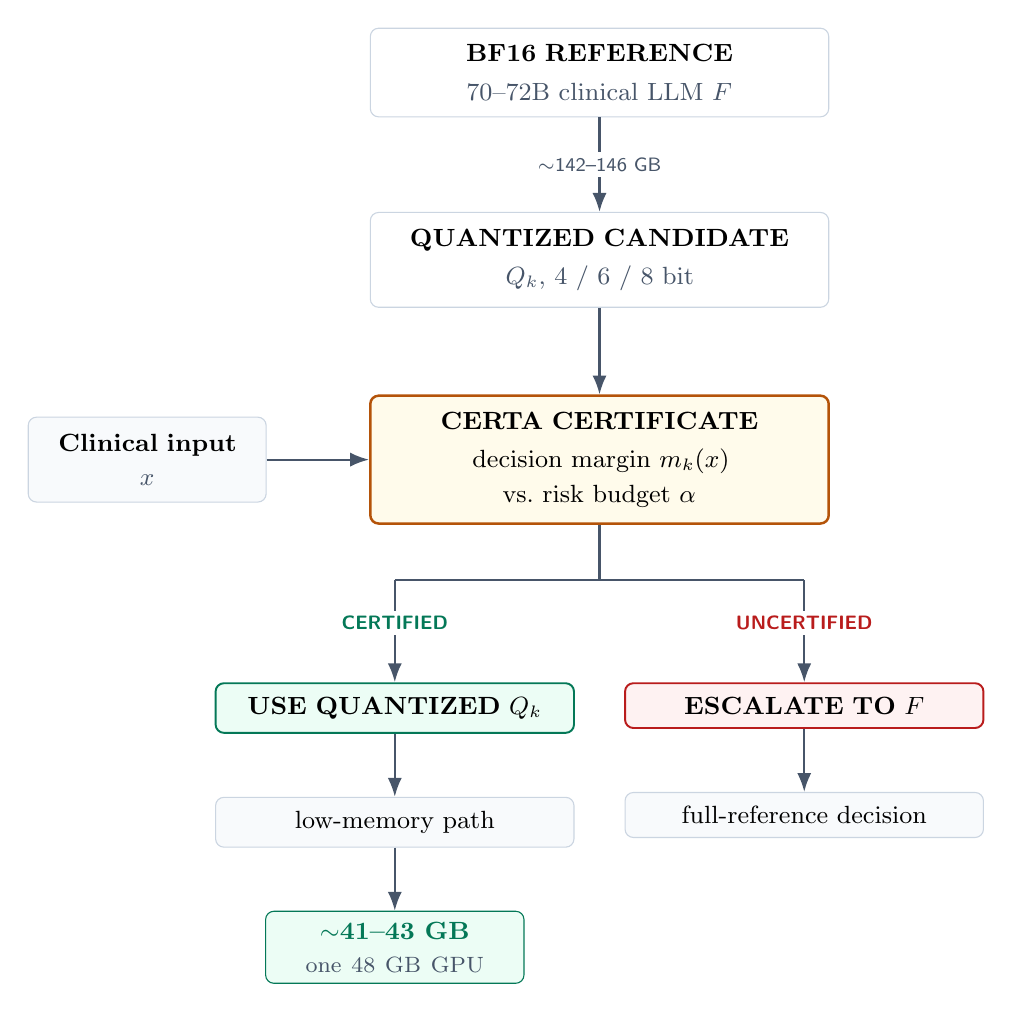
\begin{tikzpicture}[
  font=\sffamily,
  >=Latex,
  card/.style={
    draw=slate300, fill=white, rounded corners=3pt, align=center,
    text width=54mm, inner sep=6pt, font=\small},
  certaBox/.style={
    draw=amber700, fill=amber50, rounded corners=3pt, align=center,
    text width=54mm, inner sep=6pt, line width=0.9pt, font=\small},
  useBox/.style={
    draw=emerald700, fill=emerald50, rounded corners=3pt, align=center,
    text width=42mm, inner sep=5pt, font=\small, line width=0.7pt},
  escBox/.style={
    draw=rose700, fill=rose50, rounded corners=3pt, align=center,
    text width=42mm, inner sep=5pt, font=\small, line width=0.7pt},
  subCard/.style={
    draw=slate300, fill=slate50, rounded corners=3pt, align=center,
    text width=42mm, inner sep=5pt, font=\small},
  vramBadge/.style={
    draw=emerald700, fill=emerald50, rounded corners=3pt, align=center,
    text width=30mm, inner sep=4pt, font=\small\bfseries, text=emerald700},
  arr/.style={-{Latex[length=2.4mm]}, line width=0.8pt, color=slate600},
  line/.style={line width=0.8pt, color=slate600},
  lbl/.style={font=\scriptsize\sffamily, text=slate600, fill=white, inner sep=2pt},
  brlbl/.style={font=\scriptsize\sffamily\bfseries, fill=white, inner sep=2pt}
]
  % 1. BF16 reference
  \node[card] (ref) {\textbf{BF16 REFERENCE}\\[1mm]
    \textcolor{slate600}{70--72B clinical LLM $F$}};
  % 2. Quantized candidate
  \node[card, below=12mm of ref] (quant) {\textbf{QUANTIZED CANDIDATE}\\[1mm]
    \textcolor{slate600}{$Q_k$, 4 / 6 / 8 bit}};
  \draw[arr] (ref) -- node[lbl] {$\sim$142--146 GB} (quant);
  % 3. CERTA
  \node[certaBox, below=11mm of quant] (certa) {\textbf{CERTA CERTIFICATE}\\[1mm]
    decision margin $m_k(x)$\\[0.5mm] vs.\ risk budget $\alpha$};
  \draw[arr] (quant) -- (certa);
  % Side input
  \node[card, left=13mm of certa, text width=26mm, fill=slate50] (input)
    {\textbf{Clinical input}\\[0.5mm]\textcolor{slate600}{$x$}};
  \draw[arr] (input) -- (certa);
  % Fork
  \coordinate (fork)      at ($(certa.south) + (0,-7mm)$);
  \coordinate (forkLeft)  at ($(fork) + (-26mm,0)$);
  \coordinate (forkRight) at ($(fork) + ( 26mm,0)$);
  \draw[line] (certa.south) -- (fork);
  \draw[line] (forkLeft) -- (forkRight);
  % 4. Certified branch (left)
  \node[useBox, below=13mm of forkLeft] (use) {\textbf{USE QUANTIZED $Q_k$}};
  \draw[arr] (forkLeft) -- node[brlbl, text=emerald700, pos=0.42] {CERTIFIED} (use);
  % 5. Escalate branch (right)
  \node[escBox, below=13mm of forkRight] (esc) {\textbf{ESCALATE TO $F$}};
  \draw[arr] (forkRight) -- node[brlbl, text=rose700, pos=0.42] {UNCERTIFIED} (esc);
  % 6. Destinations
  \node[subCard, below=8mm of use]  (lowmem)  {low-memory path};
  \draw[arr] (use) -- (lowmem);
  \node[subCard, below=8mm of esc]  (fullref) {full-reference decision};
  \draw[arr] (esc) -- (fullref);
  % 7. Final VRAM target
  \node[vramBadge, below=8mm of lowmem] (vramEnd) {$\sim$41--43 GB\\[0.3mm]
    \textcolor{slate600}{\footnotesize\mdseries one 48 GB GPU}};
  \draw[arr] (lowmem) -- (vramEnd);
\end{tikzpicture}
}
\caption{\textbf{CERTA turns compression into a per-decision certify-or-escalate policy.}
For each clinical input $x$, the quantized candidate $Q_k$ (at $4$, $6$ or $8$ bits) proposes a
decision, and CERTA compares its decision margin $m_k(x)$ against a threshold calibrated to a risk
budget $\alpha$. Decisions that clear the certificate are served by $Q_k$ on the low-memory path;
the rest are escalated to the BF16 reference $F$. The $70$--$72$B reference occupies
$\sim$$142$--$146$\,GB and spans two $80$\,GB accelerators, whereas the certified NF4 path occupies
$\sim$$41$--$43$\,GB and fits a single $48$\,GB accelerator. For a clinical accept/reject decision
the threshold is calibrated separately per decision class (class-conditional, Mondrian).}
\label{fig:architecture}
\end{figure}


\begin{figure}[t]
\centering
\includegraphics[width=\textwidth]{fig2.pdf}
\caption{\textbf{Decision certification across eleven models, the gap between raw agreement and what
is statistically certifiable, and the resulting hardware footprint.}
\textbf{a}, Marginal certified coverage (\%) for each model under round-to-nearest at $8$, $6$ and $4$ bits,
$8$-bit LLM.int8() (INT8) and NF4 $4$-bit, at $\alpha=5\%$; the class-conditional (Mondrian) policy
used for clinical deployment is shown separately in Fig.~\ref{fig:risk} and Table~\ref{tab:frontier}. Eight-bit round-to-nearest certifies at
least $99.4\%$ for every model, whereas round-to-nearest $4$-bit is strongly model-dependent. Stars
mark configurations that certify at $100\%$ with no escalation; crosses mark the LLM.int8()
configurations that fail on bfloat16-native $70$B checkpoints, which the certificate flags as zero
coverage.
\textbf{b}, Raw decision preservation versus certified coverage for every model at round-to-nearest
$4$-bit (circles) and NF4 $4$-bit (squares), coloured by family. Points lie below the identity line
because the certificate rejects the low-margin cases that raw agreement would accept; the mean gap
is $14.8$ percentage points (for example Llama-3-8B at round-to-nearest $4$-bit, raw $70.6\%$ but
certified $15.0\%$).
\textbf{c}, Measured peak VRAM for each of the seven $70$--$72$B models at bfloat16 (BF16), $8$-bit
LLM.int8() (INT8) and NF4 $4$-bit; the three shaded regions mark how many accelerators the footprint
requires. Every model moves from $\sim$$142$--$146$\,GB at BF16, which spans two $80$\,GB GPUs, to
$\sim$$41$--$43$\,GB under NF4, which fits a single $48$\,GB device.}
\label{fig:landscape}
\end{figure}

\begin{figure}[t]
\centering
\includegraphics[width=\textwidth]{fig3.pdf}
\caption{\textbf{A risk budget determines the deployable footprint, the certificate is calibrated,
and the class-conditional guarantee costs little.}
\textbf{a}, Class-conditional deployment size as a function of the risk budget $\alpha$ for six
representative models; the curves are smooth and monotonic, and Qwen2.5-72B and HuatuoGPT-o1-72B
approach the $4$-bit floor ($25\%$, dotted) as $\alpha$ relaxes.
\textbf{b}, Calibration diagnostic: for every model and quantizer (light lines), the disagreement
observed on the held-out test set at the deployed operating point stays at or below the target
$\alpha$ (dashed identity) for $\alpha\le5\%$; the only excursions into the shaded region are
Med42-70B at $\alpha=9$--$10\%$, within the confidence slack of the procedure.
\textbf{c}, Deployment size at $\alpha=5\%$ under the marginal certificate versus the class-conditional
(Mondrian) policy. The per-class guarantee changes size by $-0.8$ to $+7.9$ percentage points (median $+2.3$); three
models escalate their entire reject class rather than certify it unsafely (labelled), and the
flagship models remain near $26\%$.}
\label{fig:risk}
\end{figure}

\begin{figure}[t]
\centering
\includegraphics[width=0.92\textwidth]{fig4.pdf}
\caption{\textbf{The quantizer determines whether four-bit compression is certifiable.}
\textbf{a}, Raw $4$-bit decision preservation moving from round-to-nearest (open circles) to NF4
(filled, coloured by family) for each model; NF4 improves preservation for all eleven models.
\textbf{b}, Certified coverage at $\alpha=5\%$ for the same models moving from round-to-nearest
(open circles) to NF4 (filled) at $4$-bit; NF4 lifts certified coverage into the $82.2\%$ to $100\%$
range (dotted line, $95\%$). The domain fine-tunes that round-to-nearest had failed, OpenBioLLM-70B
($98.1\%$), Med42-70B ($97.5\%$), MMed-Llama-3.1-70B ($96.9\%$) and BioMistral-7B ($95.8\%$), all
certify at high coverage under NF4, and MMed-Llama-3-8B rises from $0\%$ to $84.2\%$. Both panels
share the same row order, so a model can be tracked across them.}
\label{fig:quantizer}
\end{figure}

\begin{figure}[t]
\centering
\includegraphics[width=\textwidth]{fig5.pdf}
\caption{\textbf{The deployed configurations preserve external task accuracy, which is complementary
to, not the same as, reference agreement.}
\textbf{a},\textbf{b}, Disease named-entity F1 against human annotations on BC5CDR-Disease
(\textbf{a}) and NCBI-Disease (\textbf{b}) in BF16, round-to-nearest $8/6/4$-bit and the
deployed NF4 $4$-bit configuration. Eight- and six-bit change F1 negligibly; the deployed NF4 $4$-bit
configurations preserve F1 as well as or better than round-to-nearest $4$-bit (mean absolute change
$0.045$ on BC5CDR and $0.039$ on NCBI), and MMed-Llama-3.1-70B, the worst round-to-nearest $4$-bit
casualty ($-0.172$ and $-0.207$), recovers under the deployed NF4 configuration ($+0.057$ and
$+0.077$).
\textbf{c}, NF4 $4$-bit certified coverage versus the mean absolute change in F1. The per-model
association is weak and the eleven configurations occupy distinct positions: the certificate concerns agreement with the reference on the
verifier task, whereas the benchmark concerns correctness against human labels on a different task,
so the two provide complementary evidence.}
\label{fig:external}
\end{figure}


\bibliography{sn-bibliography}% common bib file
%% if required, the content of .bbl file can be included here once bbl is generated
%%\input sn-article.bbl
\clearpage
\end{document}
